% TikZ plot for 2025_linearizenn_2024
% Generated automatically with embedded data
% Requires: \usepackage{pgfplots} \pgfplotsset{compat=1.18}

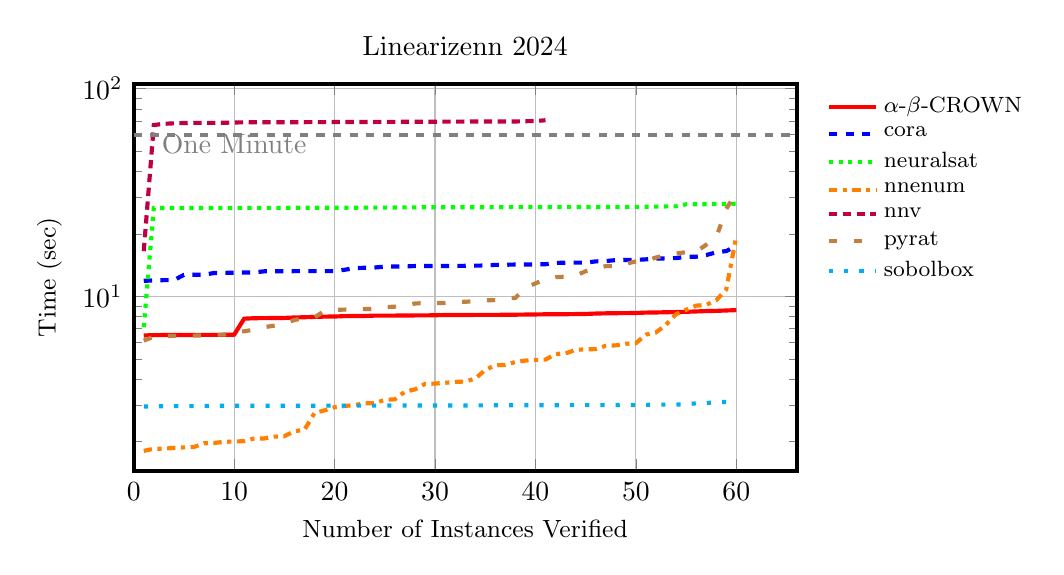
\begin{tikzpicture}
\begin{semilogyaxis}[
    xlabel={Number of Instances Verified},
    ylabel={Time (sec)},
    legend pos=outer north east,
    grid=major,
    width=10cm,
    height=6.5cm,
    ymin=1.441,
    ymax=105.7,
    xmin=0,
    xmax=66,
    line width=1.5pt,
    legend style={font=\footnotesize, cells={anchor=west}, draw=none},
    xlabel style={font=\small},
    ylabel style={font=\small},
    title={Linearizenn 2024},
    title style={font=\normalsize}
]

\addplot[color=red, mark=none, solid] coordinates {
    (1,6.477951)
    (2,6.501893)
    (3,6.508688)
    (4,6.510266)
    (5,6.515218)
    (6,6.515584)
    (7,6.517969)
    (8,6.519975)
    (9,6.524356)
    (10,6.535277)
    (11,7.806354)
    (12,7.846396)
    (13,7.851251)
    (14,7.864059)
    (15,7.869532)
    (16,7.909582)
    (17,7.931445)
    (18,7.956854)
    (19,7.985465)
    (20,7.992930)
    (21,8.028249)
    (22,8.037823)
    (23,8.039808)
    (24,8.071769)
    (25,8.075420)
    (26,8.075496)
    (27,8.085822)
    (28,8.090099)
    (29,8.091678)
    (30,8.107189)
    (31,8.124594)
    (32,8.129353)
    (33,8.131069)
    (34,8.136247)
    (35,8.136436)
    (36,8.138836)
    (37,8.149449)
    (38,8.155265)
    (39,8.167941)
    (40,8.177704)
    (41,8.192778)
    (42,8.194889)
    (43,8.198739)
    (44,8.212825)
    (45,8.223345)
    (46,8.258308)
    (47,8.280702)
    (48,8.293261)
    (49,8.298915)
    (50,8.311821)
    (51,8.348380)
    (52,8.358837)
    (53,8.382330)
    (54,8.395096)
    (55,8.421906)
    (56,8.454816)
    (57,8.491309)
    (58,8.508429)
    (59,8.546012)
    (60,8.579123)
};
\addlegendentry{$\alpha$-$\beta$-CROWN}

\addplot[color=blue, mark=none, dashed] coordinates {
    (1,11.874780)
    (2,11.922892)
    (3,11.964480)
    (4,11.968669)
    (5,12.685778)
    (6,12.702960)
    (7,12.706637)
    (8,12.952014)
    (9,12.968708)
    (10,12.995351)
    (11,13.026844)
    (12,13.036662)
    (13,13.195593)
    (14,13.206151)
    (15,13.214277)
    (16,13.215866)
    (17,13.217664)
    (18,13.217697)
    (19,13.222075)
    (20,13.225150)
    (21,13.423083)
    (22,13.672758)
    (23,13.725986)
    (24,13.764336)
    (25,13.905736)
    (26,13.910238)
    (27,13.924878)
    (28,13.988043)
    (29,13.988925)
    (30,13.994228)
    (31,13.999943)
    (32,14.003184)
    (33,14.025093)
    (34,14.049426)
    (35,14.073224)
    (36,14.170300)
    (37,14.191254)
    (38,14.225855)
    (39,14.227041)
    (40,14.243668)
    (41,14.279238)
    (42,14.478821)
    (43,14.524948)
    (44,14.530207)
    (45,14.530787)
    (46,14.731471)
    (47,14.781890)
    (48,14.945883)
    (49,14.951170)
    (50,14.977359)
    (51,15.067896)
    (52,15.209822)
    (53,15.227284)
    (54,15.285060)
    (55,15.490310)
    (56,15.517194)
    (57,15.798951)
    (58,16.294580)
    (59,16.515056)
    (60,17.496768)
};
\addlegendentry{cora}

\addplot[color=green, mark=none, dotted] coordinates {
    (1,7.106885)
    (2,26.617186)
    (3,26.619254)
    (4,26.620300)
    (5,26.625175)
    (6,26.630436)
    (7,26.631657)
    (8,26.634025)
    (9,26.634079)
    (10,26.649925)
    (11,26.660064)
    (12,26.660627)
    (13,26.664883)
    (14,26.670139)
    (15,26.674618)
    (16,26.699281)
    (17,26.704084)
    (18,26.704149)
    (19,26.715115)
    (20,26.723208)
    (21,26.725857)
    (22,26.726924)
    (23,26.729814)
    (24,26.735604)
    (25,26.740785)
    (26,26.788310)
    (27,26.819833)
    (28,26.827831)
    (29,26.840350)
    (30,26.841380)
    (31,26.853778)
    (32,26.855893)
    (33,26.856505)
    (34,26.860362)
    (35,26.860788)
    (36,26.884517)
    (37,26.890589)
    (38,26.902863)
    (39,26.907990)
    (40,26.912717)
    (41,26.913101)
    (42,26.914519)
    (43,26.915391)
    (44,26.919070)
    (45,26.935962)
    (46,26.936629)
    (47,26.937654)
    (48,26.945264)
    (49,26.947846)
    (50,26.963220)
    (51,26.998791)
    (52,27.045384)
    (53,27.102554)
    (54,27.129256)
    (55,27.745287)
    (56,27.746926)
    (57,27.780408)
    (58,27.835046)
    (59,27.837134)
    (60,27.904648)
};
\addlegendentry{neuralsat}

\addplot[color=orange, mark=none, dashdotted] coordinates {
    (1,1.801715)
    (2,1.843674)
    (3,1.845620)
    (4,1.861851)
    (5,1.872262)
    (6,1.880020)
    (7,1.960142)
    (8,1.966282)
    (9,1.992508)
    (10,1.997547)
    (11,2.006252)
    (12,2.066929)
    (13,2.067449)
    (14,2.108382)
    (15,2.118484)
    (16,2.240112)
    (17,2.276619)
    (18,2.741481)
    (19,2.822943)
    (20,2.922905)
    (21,2.962443)
    (22,2.995178)
    (23,3.051047)
    (24,3.057851)
    (25,3.170045)
    (26,3.190943)
    (27,3.473108)
    (28,3.560390)
    (29,3.783223)
    (30,3.799760)
    (31,3.831447)
    (32,3.871665)
    (33,3.885896)
    (34,4.011502)
    (35,4.419320)
    (36,4.651502)
    (37,4.673160)
    (38,4.826062)
    (39,4.903313)
    (40,4.940862)
    (41,4.954301)
    (42,5.277624)
    (43,5.306456)
    (44,5.521579)
    (45,5.553475)
    (46,5.568995)
    (47,5.777184)
    (48,5.803978)
    (49,5.909161)
    (50,5.946210)
    (51,6.541339)
    (52,6.697623)
    (53,7.302137)
    (54,8.203618)
    (55,8.610141)
    (56,9.018405)
    (57,9.086970)
    (58,9.567652)
    (59,10.804516)
    (60,19.515830)
};
\addlegendentry{nnenum}

\addplot[color=purple, mark=none, densely dashed] coordinates {
    (1,16.508426)
    (2,66.847709)
    (3,67.766875)
    (4,68.112106)
    (5,68.372691)
    (6,68.478652)
    (7,68.489288)
    (8,68.497916)
    (9,68.511339)
    (10,68.758993)
    (11,68.863098)
    (12,68.895776)
    (13,68.898460)
    (14,68.899985)
    (15,68.908078)
    (16,68.990063)
    (17,68.994410)
    (18,69.008035)
    (19,69.066612)
    (20,69.091674)
    (21,69.157848)
    (22,69.167320)
    (23,69.175295)
    (24,69.186204)
    (25,69.233236)
    (26,69.238782)
    (27,69.294971)
    (28,69.305380)
    (29,69.334373)
    (30,69.361030)
    (31,69.388290)
    (32,69.389592)
    (33,69.464129)
    (34,69.464823)
    (35,69.473914)
    (36,69.481844)
    (37,69.500238)
    (38,69.523514)
    (39,69.744473)
    (40,69.855136)
    (41,70.478456)
};
\addlegendentry{nnv}

\addplot[color=brown, mark=none, loosely dashed] coordinates {
    (1,6.115058)
    (2,6.395006)
    (3,6.427084)
    (4,6.446575)
    (5,6.452552)
    (6,6.468110)
    (7,6.480310)
    (8,6.539258)
    (9,6.539519)
    (10,6.775108)
    (11,6.781952)
    (12,6.912127)
    (13,7.103144)
    (14,7.223153)
    (15,7.363205)
    (16,7.694327)
    (17,7.843249)
    (18,7.920267)
    (19,8.516113)
    (20,8.596827)
    (21,8.629840)
    (22,8.662863)
    (23,8.682875)
    (24,8.690033)
    (25,8.870217)
    (26,8.915455)
    (27,9.029275)
    (28,9.236265)
    (29,9.278678)
    (30,9.284493)
    (31,9.294156)
    (32,9.393385)
    (33,9.409792)
    (34,9.478914)
    (35,9.562917)
    (36,9.587546)
    (37,9.738000)
    (38,9.830366)
    (39,11.002212)
    (40,11.539807)
    (41,12.114168)
    (42,12.364316)
    (43,12.436694)
    (44,12.573917)
    (45,13.206391)
    (46,13.630025)
    (47,13.969860)
    (48,13.989994)
    (49,14.337306)
    (50,14.727575)
    (51,14.790679)
    (52,15.386385)
    (53,15.765232)
    (54,16.069071)
    (55,16.322019)
    (56,16.379231)
    (57,17.718283)
    (58,19.201131)
    (59,26.384541)
    (60,31.511812)
};
\addlegendentry{pyrat}

\addplot[color=cyan, mark=none, loosely dotted] coordinates {
    (1,2.948189)
    (2,2.948840)
    (3,2.955884)
    (4,2.956773)
    (5,2.957947)
    (6,2.958985)
    (7,2.967431)
    (8,2.967748)
    (9,2.969359)
    (10,2.969795)
    (11,2.969884)
    (12,2.970613)
    (13,2.970661)
    (14,2.970852)
    (15,2.971574)
    (16,2.972236)
    (17,2.972442)
    (18,2.972502)
    (19,2.973262)
    (20,2.973859)
    (21,2.974051)
    (22,2.975399)
    (23,2.975793)
    (24,2.975894)
    (25,2.976811)
    (26,2.977864)
    (27,2.977868)
    (28,2.977871)
    (29,2.979282)
    (30,2.979952)
    (31,2.980745)
    (32,2.980932)
    (33,2.981158)
    (34,2.982839)
    (35,2.985150)
    (36,2.985412)
    (37,2.985916)
    (38,2.986123)
    (39,2.986167)
    (40,2.987496)
    (41,2.988495)
    (42,2.988748)
    (43,2.990380)
    (44,2.990488)
    (45,2.991198)
    (46,2.992362)
    (47,2.993425)
    (48,2.993767)
    (49,2.996937)
    (50,2.997895)
    (51,2.999619)
    (52,3.007335)
    (53,3.007370)
    (54,3.008908)
    (55,3.016875)
    (56,3.052659)
    (57,3.059275)
    (58,3.093073)
    (59,3.099600)
    (60,3.105665)
};
\addlegendentry{sobolbox}

% Timeout line
\addplot[color=gray, dashed, mark=none, domain=0:66] {60};

% Add timeout label as text below the line
\node[color=gray] at (axis cs:10,54.0) {One Minute};

\end{semilogyaxis}
\end{tikzpicture}
